\documentclass[9pt,a4paper]{acmproc}
\usepackage[utf8]{inputenc}
\usepackage{amsmath}
\usepackage{amsfonts}
\usepackage{amssymb}
\usepackage{graphicx}
\usepackage[english]{babel}
\usepackage[utf8]{inputenc}
\usepackage{amsmath}
\usepackage{cite}

\graphicspath{}

\author{
  \texttt{Theodor Fleming}
  \and
  \texttt{Andreas Nordberg}
}

\begin{document}
\pagenumbering{gobble}

\title{%
	TDDD66 Projekt \\
	\large Wi-Fi Multicasting}
\maketitle

\clearpage
.
\clearpage

\begin{abstract}

This study explains what multicast is, specifically using Wi-Fi, and where and when to use it. The report briefly compares how similar services, such as unicast, work and differentiate from each other. The conclusion of this study is that multicasting has an extremely nische usage. While it definetly can be used by the average home user, a well-optimized and functioning multicasting network requires a more advanced user to setup. This makes multicasting most suited in company local networks setup by someone with deeper networking knowledge.
\end{abstract}

\clearpage

\section{Inledning}

\subsection{Context}

Multicasting is a method of sharing information by communicating with a select amount of receivers. Other methods exist for this purpose, such as unicast and broadcast, but these will play a lesser role in this study and will only be compared with multicasting. There are different kinds of networks that use multicasting to distribute information, but this paper will mainly focus on how multicasting is handled with Wi-Fi. As with any means of solving a problem, different results can be expected from solving the problem using different methods. In our case with this report, how does Wi-Fi multicasting compare to other means of sharing information within a network in terms of different methods of routing? How well does multicasting do compared to other methods of routing in terms of performance? These are the kind questions this report will delve into and try to answer.  

\subsection{Motivation}

This report will cover when and where the multicasting should be used in favor of other communication services of the sort, for example unicast. The following questions then are, why isn't multicasting as widespread as unicasting and broadcasting? In what cases does the performance differ between the several options, and what is the cause of this?

\subsection{Narrow Scope}

In this study we will do tests and experiments with multicasting using a number of different devices and recievers to see how the multicasting performs in comparision to other alternatives. Apparently, multicasting comes with some benefits and disadvantages and is most useful during only some circumstances. Perhaps multicasting can be used in more areas than it currently is? We might find even more uses for the technique in this study. We hope that the result of this study will answer these questions.

\subsection{Methodology}

We will conduct tests of multicasting performance in terms of speed and reliability by using different devices, networking options and receivers. We will also compare the results of these tests by performing similar tests with unicasting, to draw a conclusion of when either of the techniques are more suited for use. To achieve this, we will try to setup some kind of multicasting enviroment to measure the values we are looking for during different circumstances.

\subsection{Gameplan}

We are going to do research to understand more how multicast is used, how it works and how we can prepare for our tests until milestone 2. We will probably need to understand and get a better feel for multicast before we can start with our tests. After that we are going to perform and draw conclusions from our experiments until milestone 3 and fill the report with more facts about multicast used with Wi-Fi, pros, cons and comparison with other communication services. Now we are going to prepare for the seminar presentation, get feedback and fix the report until final report.

\newpage

\section{Background}

\subsection{What is multicasting?}

While a brief explanation was given in the introduction, we feel like a clarification is needed. With multicasting you are typically referring to the use of multicasting in the network layer protocol, also called IP multicasting. When we started this project, we ourself initially thought that multicasting was the process of multicasting a message on the physical layer, e.g. in our case with Wi-Fi multicasting, perhaps a password-protected network where only the select few connected to the wireless network would be able to decipher and read the outgoing frames sent from the access point out of everyone within the vicinity who could detect them, which would make out a multicast network. This is naturally not how multicasting really works.
\subsubsection*{2.1.1 Unicast}

When you explore internet you are most likely to use unicast messaging, it is used when there is a single destination node. 

\begin{figure}[h!]
  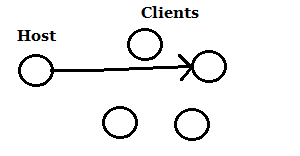
\includegraphics[width=\linewidth]{unicast.png}
  \caption{Unicast}
  \label{fig:Unicast}
\end{figure}

\subsubsection*{2.1.2 Broadcast}

The contrast of unicast is broadcast where the destination is all the nodes in the network, for example used when your mobile device is searching for a Wi-Fi hotspot.
\begin{figure}[h!]
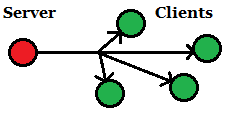
\includegraphics[width=\linewidth]{broadcast.png}
\caption{Broadcast}
\label{fig:Broadcast}
\end{figure}

\subsubsection*{2.1.3 Multicast}

Multicasting is actually the act of transmitting information in the form of “multicast packets”. These packets are actually pretty similar to the standard unicast packets, commonly referred to as network packets, but they differ in some ways. While a unicast packet always has one address assigned to a respective receiver, multicast packets have one or more addresses, or a group address which delivers the information to every destination. This is also why multicasting is commonly referred to as “IP multicasting”, because this process is handled at the Network Layer. The perhaps obvious pro to this method of distributing information is that only one sent message or frame is required to share a piece of data to multiple receivers, as opposite to one packet times the number of receivers by using unicasting. A huge chunk of bandwidth can be saved this way, the user can expect its information to be delivered to their device faster and lots of energy and resources can be potentially saved using this method of distribution.
	
	\begin{figure}[h!]
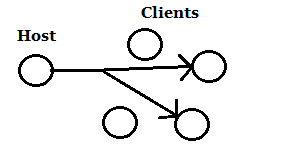
\includegraphics[width=\linewidth]{multicast.png}
\caption{Multicast}
\label{fig:Multicast}
\end{figure}

	These pros sounds great, right? Then why aren’t we using multicasting over the place? Well, multicasting has its cons as well. In our case with Wi-Fi multicasting, while the sender establishes a stable connection with the wireless access point in which the AP acknowledges every received message, the same is not done between the access point and the multiple receivers in the actual multicasting proccess. Much like the UDP protocol, there is no guarantee that a multicasted message is delivered to the designated destination, because the receiver doesn’t reply with any acknowledgement of receiving the given message. \cite{udpSource}
	
	There’s also another con to be considered when you’d want to use multicasting in a network. If there is one or more receivers in the multicast network who are slower than the rest of the receivers in the network, for example if this receiver is utilizing a Wi-Fi power saving mode, the entire multicasting network is slowed down to adjust to this one, or more, users. For example, in the case of the power saving mode, several frames are buffered at the access point. DTIM (Delivery Traffic Indicator Message) are then included with the frames to be multicasted, which are a sort of timer of when the access point should release its buffer to all the recipients and not only the ones who have the power save mode enabled. The DTIM included in the frames makes the receivers aware of when to “wake up” from their power saving mode and be ready to receive the buffered batch of frames. \cite{impMult} 
However, for this study we assume that no Wi-Fi power saving mode is used. These pros and cons raises the question of when exactly multicasting would be preferred over unicasting.
\newline
\newline



\subsection{Multicasting History}

The year was early 1980 and the Stanford University student Steve Deering was tasked with developing a distributed operating system. It was to be called Vsystem and consisted of a few number of computers able to communicate with eachother using a single ethernet segment. This way the computers could collectively solve tasks together. The system allowed one of the computers in the network to send messages to the rest of the group via MAC layer multicasting. This method of distributing information to several computers at once was nothing short of a success and the need for more computers to be added to this multiprocessing system arose. The problem they faced then was that the other computers available to them was located at the other side of the campus, separated by multiple routers in between the networks. As a result the system had to be extended to allow operation on the layer 3 of the OSI reference model so that the other computers could participate in the multiprocessing system. Steve Deerling then used existing technologies to develop a new distance vector-based multicast routing protocol suited to the system he had imagined, which led into further research about IP multicasting. \cite[s.~7]{briefHist}


\subsection{Experiment}

We are going to use a network simulating program such as one Cisco can provide us with to simulate a network where we compare multicast performance with unicast. By doing this we hope to find out when it's worth implementing multicast instead of unicast. We are going to start in a small scale and see if there is any difference in bandwidth depending on either you use multicast or unicast. Then we are successively going to increase the size of the network to see when you reach the point where the multicast technology is using less bandwidth and increasing the speed of the data that is sent within the network.
We also want to try and see if we can create our own multicast network within our home. This could maybe be in favour for example if you have two computers in different parts of your house and you want to play the same song on them simultaneously. We are not really sure on how this is going to be done at this point of time in the project but the basics are that we need to connect these devices over the same IP address. You could compare it with a walkie talkie where everyone on a specific channel can communicate with everyone except in this case the channel is replaced with an IP address. We have to allocate the same a class D IP address to each device in the network that we can call the group address.

\subsubsection{Multicast group}

The device that wants to send and receive multicast datagrams must be in a multicast group. These groups are on a particular network interface and have the IP multicast-address of class D. The range of the D-classified IP address is from 240.0.0.0 to 239.255.255.255. Basically you allocate the device that you want to send and receive multicast datagrams from and to a specific class D address. Now the device knows that if a datagram is sent to that specific IP address it wants to explore it further by sending it up to the next layer. And same thing for the host when it sends the multicast datagram it as to send it to a established class D address. This is what you call IP multicasting and it is what we are mostly going to investigate but there is also something called hardware/ethernet multicasting. The main difference between these two multicasting techniques is that IP Multicasting is using the IP address to tell a unicast, multicast and broadcast apart while the hardware multicasting is looking at the MAC address. When a normal packet is sent it is probably sent using unicast and the MAC source address is the actual MAC address of the source. But when a multicast datagram is sent the MAC source is not the MAC source of the real source, it is a multicast MAC source that the other devices in the multicast group knows. The way it tells the difference is by the first number in the MAC address. Say our computers MAC address is D4:3D:7E:9C:0C:86. If we take a look at the first number, D4 and convert it from hexadecimal to binary we get 1101 0100 and the last number is a 0 there, the last one i 0100. That tells the device that it is not a multicast MAC address, but if it would have been a 1 instead of a 0 then it would have been a multicast MAC address. For example if the MAC address was 01:00:5E:00:00:00 and once again we take a look at the first number, 01. Convert it from hexadecimal to binary and we get 0000 0001, a one as the last number which tells us it is a MAC address for multicasting.

When we will try to set up our own multicast network at home we are going to use a program that tests if multicast messages is being transmitted and received. It works such as you decide which nodes, in this case devices on the network, that will send multicast datagrams and which nodes that will receive the multicast datagrams. By starting very basic we can quickly test if our multicast network is functionally and then move on to more difficult tasks. As we mentioned before about playing music on two computers at the same time, this is a goal that we would be really happy if we succeeded to accomplish. This might require more work and knowledge than we think but it is still our goal. We are happy if we just succeed with sending a message to all computers in the multicast network at the same time, creating our own sms group over the computers in the network.

We believe that it really depends on what you send within the network that decides if multicast or unicast should be used more than the size of the network. Imagine just sending out a message saying “Merry Christmas!” to everyone's computer in the office. That would not take much bandwidth even if it was sent using unicast and therefore multicast would not be needed. But if we have the same scenario but instead we send a live stream that greets merry Christmas, then a lot of the bandwidth would have been allocated for that stream. If we instead use multicast in the second scenario the bandwidth would have been the same as if only one was watching the stream and a lot of bandwidth would have been saved. So we have to look at both what is sent and how many it is sent to before deciding whether to use multicast or unicast. We also think that with today's technology unicast is probably the best to use in most cases and multicast only in some rare situations. \cite{multExplained} \cite{whatIsMult} \cite{understandIpMult} 


\clearpage

\section{Results}

\subsection{What we found out in the study}

When we first started out with this project we thought it would be a lot easier to implement a Wi-Fi, or a wired, multicast network at home or in a simulation program than it turned out to be. The only multicasting service that worked from the get-go without any issues at the start of our study was a simple program made for multicast testing. With this program you could choose whether if you want a device to send or receive multicast packets for a specific multicast group on the network which also ran the same application. We ran this program on several computers at the same time while we traced the packets to see if we could use any information in these packets for our study. The trace showed that the multicasting packets were of UDP type and the time they were received and sent. We concluded that this information was not going to be of any use for us in this study, but it did confirm everything we already knew about multicast packets.

Since multicast networks are so uncommon and hard to come by we later felt the need to simulate these networks instead of implementing one of our own. While it’s obviously not impossible to create a multicast network, we did not have the knowledge or experience to do so at this point of the project. We found out that creating a native multicasting network required a lot of experience with routers and networking applications. We tried alot of different simulation programs but they were simply too advanced for us perform tests with, or to even setup. Even though we managed to simulate a working ethernet multicasting network using an existing template, we were again not able to perform the tests we wanted to retrieve the exact data we wanted from network. Some of them required you to program the networks in programming languages unknown to us, and some did not have the functionality we were looking for to set up a Wi-Fi multicasting network to perform the tests on. Also, none of the simulators we found could simulate any circumstances of using Wi-Fi multicasting in real life to our knowledge, e.g. some other signal interfering with the Wi-Fi multicast signals.
Although we did find one suitable simulation progam named eNSP in which we could simulate a movie being streamed from one server, through a router, to the clients using multicast. The simulation we performed was not in a wireless network using Wi-Fi since they program did not support wireless multicasting to our knowledge. In the simulation we configured the server to send a stream with a D-classified IP-address as the destination. The packets were sent to the switch using TCP-packets. When the packets arrived at the switch they were converted into UDP-packets and distibuted to all connected clients that had joined the Multcast group using same IP-address as the destination. The movie was successfully played at the server and streamed to the clients with a slight delay because of the round trip time.

As the project was coming to a close, we came across the multicasting function of the media player VLC. In hindsight we really wish we would have found out about this one sooner. With this tool we could easily setup a live authentic Wi-Fi multicasting network to stream media from one acting server device, through a wireless access point, to multiple receivers within a network. While we didn’t have the time to perform the full scale tests we initially intended to using this setup we could still get some results out of it, benefiting our study.
When we got our sample video to play on the different receiving hosts using multicasting, the qualities of the playbacks were varied. If we opened a second instance of VLC for playback on the server device, the quality of the playback was decent, with little visual artifacts and audio stuttering. When we opened the video stream on a second computer, the quality of the video was approximately the same as when we opened a second instance of VLC on the server, as in it had some irregular visual and audial quality drops and stuttering. When we did this on a larger scale during a presentation of our project, the playback quality was not as good as with our smaller scaled test, with regular bad visual artifacts and some frequent audio stuttering, but we didn’t really get to verify this with everyone who helped us out with this test. Finally, as we tried to use the VLC Android application to receive the multicast video stream. This went horribly. Out of many, many attempts we only got video to play a few times, and audio to always work but with frequent stuttering.

\subsection{Discussion}
It’s no surprise we don’t see Wi-Fi multicasting often being used by regular consumers. This is because multicasting, Wi-Fi multicasting even more so, is not very developed for the every day user since it apparently has a such a nische usage. The reason to that might be because the average user simply doesn't need multicast, because of regular unicasting can serve the purpose of distributing data just as well. Say an average user want to play a movie, located on a computer, on his phone. He would likely think of transfering the the entire file to the other device using a unicast method instead of streaming it live to his phone using multicast.
Companies on the other hand might be interested of implementing Multicast in a network to save bandwidth or for the sake of simplicity, providing they would often send the same data to several destinations at the same time. For example, a use of multicasting for a company might be to setup several screens to show the same video wirelessly within a limited area, or to use several wireless speakers to play the same song. A company would probably also have access to people with deeper networking knowledge to make this multicasting network function well, without any visual artifacts or audio stuttering.

As we’ve mentioned several times in the report, one of our first goals were to setup our own local ulticast Wi-Fi network. Even though we put a lot of time into trying to understand how to configure routers and computers to join multicast groups and other means necessary to create a multicast network, we think that it doesn’t have to be as difficult to do as it would seem. We believe that if some development was put into making multicasting more user-friendly it wouldn’t have to be harder to setup and use than your traditional local or internet unicast network. We can make a comparision to one’s regular home network. It’s very easy to install a home network because there exists wizards and easy-to-use guides so that even the most inexperienced user can setup their own home network, as opposed to a dedicated Multicast network which often requires you to lookup online guides made with advanced users in mind. 

We were about to run out of time with the project when we came across the application eNSP, albeit less so than we found out VLC supported multicasting, one of the programs we tried to perform our simulation with. If it had been found at an earlier stage of the study we would probably have gotten more experience with using it and being able to retrieve some useful data. When we simulated the multicast network using eNSP we did it over a simulated wired network and not a Wi-Fi one since the program did not support it to our knowledge. 

As we mentioned earlier we came across the VLC multicasting tool even later in the study which was unfortunate because we would have wanted to trace the packets, see how large of an amount of packets that were lost, which packets was lost, among other tests that would have explained further why we got such poor playback while using the service. With our newfound knowledge about multicasting we can still use the results we got for something though. The computer to multicast its media file first and foremost sends packets to the home network’s router/wireless access point using the TCP protocol. The router receives the TCP-packets and converts them into UDP-packets, and then distributes them to the other receiving devices in the multicast group. While it worked fairly well during some circumstances we had the common issue of visual artifacts and audio stuttering, which would be the result of packet losses and the UDP-protocol not supporting any packet-loss handling. This is because UDP-oriented packets are transaction oriented, meaning that delivery is not guaranteed and the protocol doesn’t keep track of if a packet is lost. If we were to redo this study, we would perform test to get an exact number on how large of an amount of the packets were lost in a playback of a video using the VLC multicasting tool. \cite{udpSource}


\begin{figure}[h!]
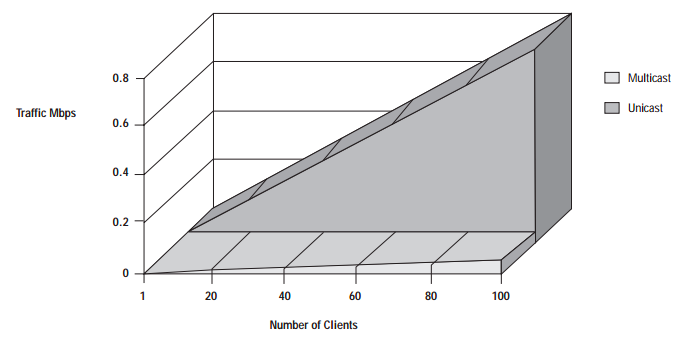
\includegraphics[width=\linewidth]{graph.png}
\caption{Graph comparing unicast and multicast}
\label{fig:graph}
\end{figure}

This figure gives a good overlook on how much bandwidth is saved by using multicast compared to using unicast in relation to an increasing number of receivers. It shows a case of a given number of clients listening to the same 8 Kbps audio stream, distributed with unicast and multicast. This was something we initially wanted to create ourselves using data from our own tests and measurements but as we’ve mentioned several times, we did not have the competence at the time needed to do this with simulation programs we attempted to use. As the graph shows, multicasting really pays off when it can be used. For example, when there's 100 clients, about 16 times less bandwidth needs to be used to transfer the exact same data to the receivers if you choose multicasting over unicasting! \cite[s.~4]{graphSource}

\subsection{Conclusion}

At the start of this project we thought that we had to and would be able to configure our home router and computer to be able to send and receive multicast packets. After weeks of research we concluded that we wouldn’t be able to do so, up until we found out how we could use VLC to conduct our study. The routing technique multicast is apparently a lot more complicated to use and operate as a standard consumer than compared to unicast and broadcast. Your phone is able to automatically connect to the strongest Wi-Fi access point using the Broadcast protocol without hassle, and within seconds you can connect to the public internet using unicast. The multicasting method is not very new, yet is still not as widely used as the other methods. This is because the average user rarely have the need to use services which applies multicasting, which results in multicast not being very common or easy to use for a regular consumer. This is something that really showed in the research we performed, since such a seemingly easy task as setting up a multicast network requires a lot more knowledge than the basics you need to have for creating a regular home network for Unicasting. Every guide and study for setting up your own well functioning multicast network assumes that you know a lot more about routers and networks than a regular consumer of internet. From the results of our study, the use of multicasting seems to be very limited and more often suited for larger local networks such as company networks.

\clearpage

\begin{thebibliography}{9}

\bibitem{impMult}
  Jim Geier,
  \emph{Implementing Wi-Fi Multicast Solutions}.
  \newline
  Published: 2004-11-09. Fetched: 2015-09-25 \newline
  URL: http://www.wi-fiplanet.com/tutorials/article.php/3433451/Implementing-Wi-Fi-Multicast-Solutions.htm
  
\bibitem{briefHist}
	Beau Williamson,
	\emph{Developing IP Multicast Networks}.
	\newline
Cisco Press; 1 edition (October 29, 1999).

\bibitem{multExplained}
  Juan-Mariano de Goyeneche,
  \emph{Multicast Explained}.
  \newline
  Published: 1998. Fetched: 2015-09-25 \newline
  URL: http://www.tldp.org/HOWTO/Multicast-HOWTO-2
  
\bibitem{whatIsMult}
  Windows Server,
  \emph{What Is IPv4 multicasting?}.
  \newline
  Fetched: 2015-09-25 \newline
  URL: https://technet.microsoft.com/en-us/library/cc772041(v=ws.10).aspx
  
  \bibitem{understandIpMult}
  Page Administrator,
  \emph{Multicast - Understand how IP multicast works}.
  \newline
  Fetched: 2015-09-25 \newline
  URL: http://www.firewall.cx/networking-topics/general-networking/107-network-multicast.html
  
  \bibitem{udpSource}
  J. Postel,
  \emph{User Datagram Protocol}.
  \newline
  Published: 1980. Fetched: 2015-10-15 \newline
  URL: https://tools.ietf.org/html/rfc768
  
   \bibitem{graphSource}
  Cisco Systems, Inc.,
  \emph{Multicast Deployment Made Easy}.
  \newline
  Published: 1999. Fetched: 2015-10-15 \newline
  URL: http://ftp.icm.edu.pl/packages/cisco-ipmulticast/whitepapers/Multicast-Deployment-Made-Easy.pdf
  
%\bibitem{randall2008}
%	Randall D. Knight,
%	\emph{Physics for Scientists and Engineers: A %Strategic Approach with Modern Physics (2nd %Edition)}.
%	\newline
%Addison-Wesley, 2a upplagan, 2008.

%\bibitem{polesAndZeros}

%	\emph{Understand Poles and Zeros}.
%	\newline
%	Publicerad 2002-11-01. Hämtat: 2015-06-01.
%	\newline
%	URL: http://web.mit.edu/2.14/www/Handouts/PoleZero.pdf

\end{thebibliography}

\end{document}
